%!TEX root = ../main.tex
\newgeometry{left=4cm}

\begin{titlepage}
	\begin{center}
	
		\includegraphics[width=.2\textwidth]{figs/portada/LogoFCyT}
		
		\Large
		\textbf{Universidad Nacional de Caaguazú}
		
		\vspace{0.3cm}
		\Large
		Facultad de Ciencias y Tecnologías
		
		\vspace{1.2cm}
		
		\textbf{\Titulo}
		
		\subTitulo
		
		\vspace{1cm}
		
		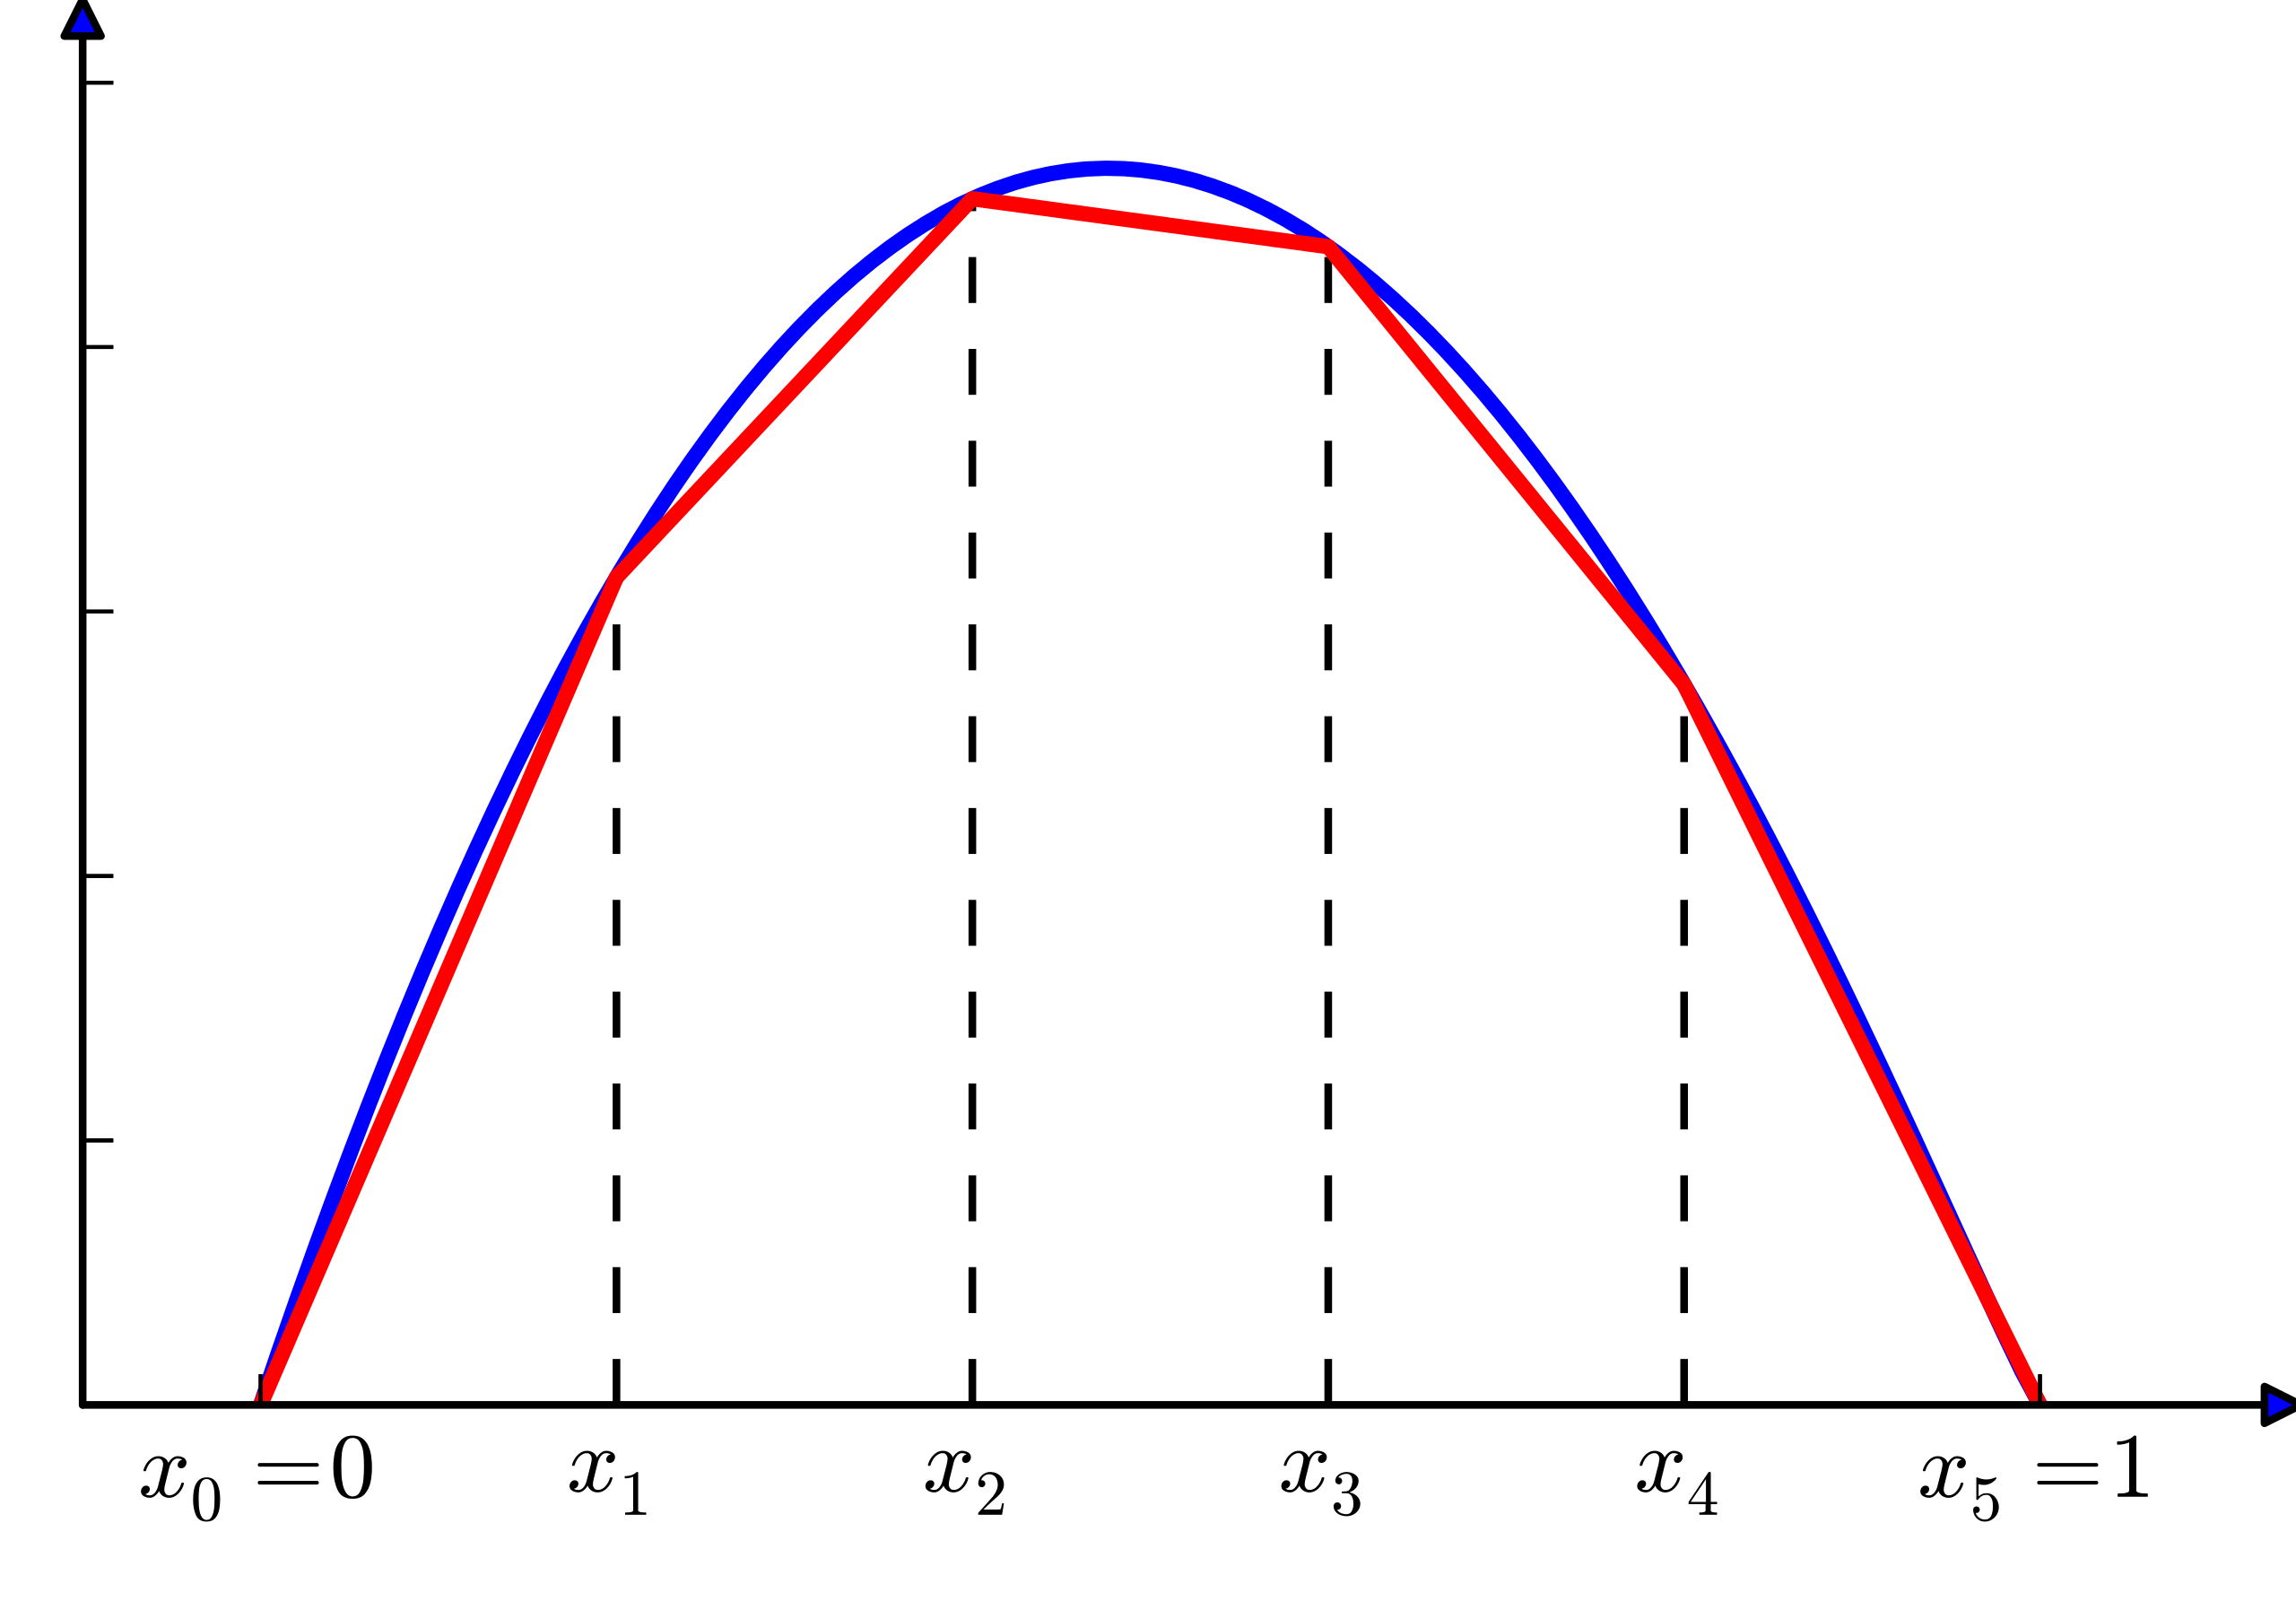
\includegraphics[width=0.4\textwidth]{figs/portada/fem}
		
		\vspace{1cm}
		
		\textbf{\yo}
		
		Ing. Civil, M.Sc.
		
		\vspace{0.8cm}
		
		\large
		Coronel Oviedo - Paraguay
		
		\fecha
		\vspace{.5cm}
		
		Material en elaboración: versión 0.1.0-alpha
	\end{center}
\end{titlepage}

\restoregeometry